\newproblem{167D. Wizards and Roads}
\begin{prob}
	给出平面上$n(n \le 10^5)$个点,保证点的分布随机,
	且任意两点$x,y$坐标均不同。
	$u,v$两点之间能连边的条件是
	$u_y > u_y$,且任何严格在点$u,v$形成的拐角中的
	点$w$,都有一个点$s$并不在$u,v$形成的拐角中,
	并且$w_x < s_x < u_x$,同时$s_y > v_y$。\par
	$u,v$形成的拐角的定义如下图阴影部分:
	\par
	{\centering
	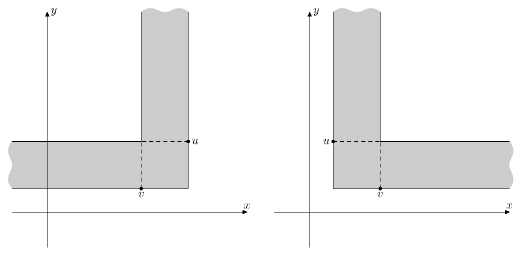
\includegraphics[scale=0.75]{167D.png} } 
	\par
	
	现在给出$m(m \le 10^5)$个询问$[L_i, R_i]$,
	表示将横坐标在$[L_i, R_i]$的点取出,按上述
	规则两边得到的无向图中的最大匹配数。

\end{prob}

\begin{sol}
	首先,需要简化连边的条件。不难发现:
	对于每个$u$,找到其右第一个纵坐标
	大于$u_y$的点$s$,那么$u$往右只能
	跟$s$左边第一个纵坐标小于$u_y$的点$v$
	连边。由于每个点最多往下连两条
	边,所以形成的图是一个以纵坐标最大的点
	为根的二叉树,且期望深度为$O(\log n)$。
	\par
	按以上规则建好树后,考虑如何回答询问。
	求树的最大匹配树容易联想到一个简单的
	dp:$f[i][0/1]$表示以$i$为根的子树中,
	$i$是否匹配的最大匹配数。递推也非常容易。\par
	但原问题还有一个限制:每次询问的树的形态
	都是不一样的。但新树可以通过以下操作得到:
	对每个在$[L_i, R_i]$内的点$x$,它的父亲
	修改为最近的一个祖先$y$,且$y$也在$[L_i, R_i]$内。
	这样修改后有一个重要的性质没有变化:即答案
	仍然可以通过合并左右子树来得到。于是,最终
	算法就是建一个类似于线段树的树,修改合并函数,
	保证合并的子树都在区间内。整个算法的复杂度为$O(m \log n)$。
\end{sol}
